%
% @author   Christopher Schmitt & Matthew Warren
% @version  3/29/2020
% @license  MIT
%


\documentclass{article}


%
% Document Imports
%

\usepackage{fancyhdr}
\usepackage{extramarks}
\usepackage{amsmath}
\usepackage{amssymb}
\usepackage{amsthm}
\usepackage{amsfonts}
\usepackage{color}
\usepackage{listings}
\usepackage[color]{register}
\usepackage{booktabs}



%
% Document Configuration
%

\newcommand{\hwAuthor}{Christopher K. Schmitt and Matthew Warren}
\newcommand{\hwSubject}{CS 358}
\newcommand{\hwSection}{Section 01}
\newcommand{\hwSemester}{Spring 2020}
\newcommand{\hwAssignment}{Progress Report 2}

\definecolor{dkgreen}{rgb}{0,0.6,0}
\definecolor{gray}{rgb}{0.5,0.5,0.5}
\definecolor{mauve}{rgb}{0.58,0,0.82}

\lstset{
  frame=tb,
  language=Verilog,
  aboveskip=3mm,
  belowskip=3mm,
  showstringspaces=false,
  columns=flexible,
  basicstyle=\ttfamily,
  numbers=none,
  numberstyle=\tiny\color{gray},
  keywordstyle=\color{blue},
  commentstyle=\color{dkgreen},
  stringstyle=\color{mauve},
  breaklines=true,
  breakatwhitespace=true,
  tabsize=3
}


%
% Document Environments
%

\setlength{\headheight}{65pt}
\pagestyle{fancy}
\lhead{\hwAuthor}
\rhead{
  \hwSubject \\
  \hwSection \\
  \hwSemester \\
  \hwAssignment
}

\newenvironment{problem}[1]{
  \nobreak\section*{#1}
}{}


%
% Document Start
%

\begin{document}
  \begin{problem}{Instruction Set Architecture}
    \paragraph{}
    We implement a 3-satge MIPS data-path which implements all R-Type instructions and ADDI.

    \begin{table}[]
      \begin{tabular}{@{}lllp{6.8cm}@{}}
        \toprule
        Instruction & Opcode & Format & Description \\ \midrule
        add & 0000 & R-Type & Adds \$rs and \$rt together using arithmetic addition, places the sum in \$rt \\
        sub & 0001 & R-Type & Subtract \$rt from \$rs, places the difference in \$rt \\
        and & 0010 & R-Type & Perform bitwise ANDing on \$rs and \$rt, place the result in \$rd \\
        or & 0011 & R-Type & Perform bitwise ORing on \$rs and \$rt, place the result in \$rd \\
        addi & 0100 & I-Type & Add \$rs to immediate value, place the result in \$rt \\
        slt & 0111 & R-Trpe & Put 0x01 in \$rd if \$rs $<$ \$rt, 0x00 otherwise \\ \bottomrule
      \end{tabular}
    \end{table}
    
    \begin{register}{H}{R-Type}{}
      \begin{center}
        \regfield[green!30]{}{4}{12}{{op}}
        \regfield[red!30]{}{2}{10}{{rs}}
        \regfield[blue!30]{}{2}{8}{{rt}}
        \regfield[orange!30]{}{2}{6}{{rd}}
        \regfield[gray!30]{}{6}{0}{{unused}}
      \end{center}
    \end{register}

    \begin{register}{H}{I-Type}{}
      \begin{center}
        \regfield[green!30]{}{4}{12}{{op}}
        \regfield[red!30]{}{2}{10}{{rs}}
        \regfield[blue!30]{}{2}{8}{{rt}}
        \regfield[orange!30]{}{8}{0}{{value}}
      \end{center}
    \end{register}

    In the above diagrams, \emph{op} is the opcode, \emph{rs} is the
    source register, \emph{rt} is the target/destination register, and
    \emph{rd} is the destination register.  Value is the immediate value
    in I-Type instructions.
  \end{problem}

  \begin{problem}{Control Table}
    \begin{table}[]
      \begin{tabular}{@{}llllllll@{}}
      Operation & RegDst & ALUSrc & MemToReg & RegWrite & MemWrite & Branch & ALUOp \\ \midrule
      add & 1 & 0 & 0 & 1 & 0 & 0 & 00 \\
      sub & 1 & 0 & 0 & 1 & 0 & 0 & 01 \\
      and & 1 & 0 & 0 & 1 & 0 & 0 & 10 \\
      or & 1 & 0 & 0 & 1 & 0 & 0 & 10 \\
      addi & 0 & 1 & 0 & 1 & 0 & 0 & 00 \\
      lw & 0 & 1 & 1 & 1 & 0 & 0 & 00 \\
      sw & 0 & 0 & 0 & 0 & 1 & 0 & 00 \\
      slt & 1 & 0 & 0 & 1 & 0 & 0 & 10 \\
      beq & 0 & 0 & 0 & 0 & 0 & 1 & 01 \\
      bne & 0 & 0 & 0 & 0 & 0 & 1 & 01
      \end{tabular}
    \end{table}
  \end{problem}

  \begin{problem}{Source Code}
    \lstinputlisting[language=Verilog, basicstyle=\scriptsize\ttfamily]{processor.vl}
  \end{problem}

  \begin{problem}{Machine Translation}
    \lstinputlisting[basicstyle=\ttfamily]{test.txt}
  \end{problem}

  \begin{problem}{Output (With Nop)}
    \begin{center}
      \begin{lstlisting}[basicstyle=\footnotesize\ttfamily]
        PC     IFID_IR                 IDEX_IR                 data
        0     xxxxxxxxxxxxxxxx        xxxxxxxxxxxxxxxx          x
        1     0000000000000000        xxxxxxxxxxxxxxxx          x
        2     0100000100001111        0000000000000000          0
        3     0100001000000111        0100000100001111         15
        4     0000000000000000        0100001000000111          7
        5     0010011011000000        0000000000000000          0
        6     0000000000000000        0010011011000000          7
        7     0001011110000000        0000000000000000          0
        8     0000000000000000        0001011110000000          8
        9     0011101110000000        0000000000000000          0
       10     0000000000000000        0011101110000000         15
       11     0000101111000000        0000000000000000          0
       12     0000000000000000        0000101111000000         22
       13     0111111001000000        0000000000000000          0
       14     0111101101000000        0111111001000000          0
       15     xxxxxxxxxxxxxxxx        0111101101000000          1
      \end{lstlisting}
    \end{center}
  \end{problem}

  \begin{problem}{Output (Without Nop)}
    \begin{center}
      \begin{lstlisting}[basicstyle=\footnotesize\ttfamily]
        PC     IFID_IR                 IDEX_IR                 data
        0     xxxxxxxxxxxxxxxx        xxxxxxxxxxxxxxxx          x
        1     xxxxxxxxxxxxxxxx        xxxxxxxxxxxxxxxx          x
        2     0100000100001111        xxxxxxxxxxxxxxxx          x
        3     0100001000000111        0100000100001111         15
        4     0010011011000000        0100001000000111          7
        5     0001011110000000        0010011011000000          X
        6     0011101110000000        0001011110000000          x
        7     0000101111000000        0011101110000000          X
        8     0111111001000000        0000101111000000          x
        9     0111101101000000        0111111001000000          X
       10     xxxxxxxxxxxxxxxx        0111101101000000          X
       11     xxxxxxxxxxxxxxxx        xxxxxxxxxxxxxxxx          x
       12     xxxxxxxxxxxxxxxx        xxxxxxxxxxxxxxxx          x
       13     xxxxxxxxxxxxxxxx        xxxxxxxxxxxxxxxx          x
       14     xxxxxxxxxxxxxxxx        xxxxxxxxxxxxxxxx          x
       15     xxxxxxxxxxxxxxxx        xxxxxxxxxxxxxxxx          x
      \end{lstlisting}
    \end{center}
  \end{problem}

  \pagebreak
  \begin{problem}{CPU Complete Diagram}
    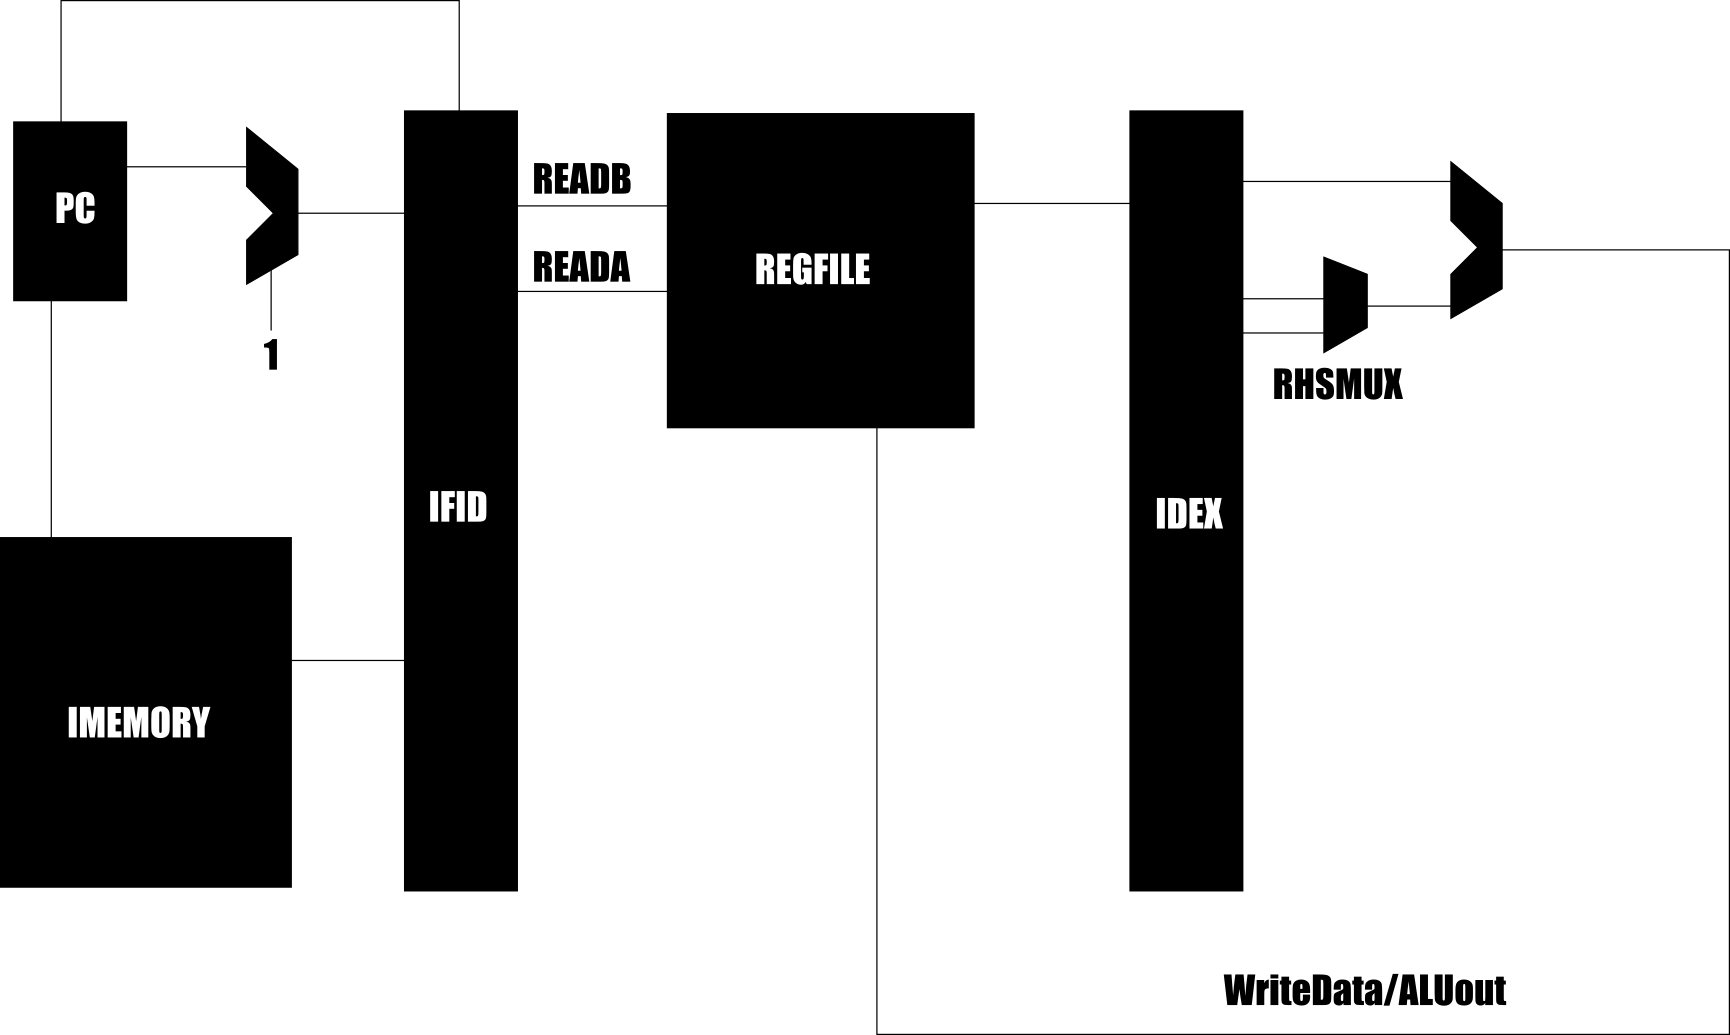
\includegraphics[scale=0.3]{text898.png}
  \end{problem}
\end{document}